\chapter{Experimental results}
\label{chap:chap3}
\textit{In this section we will detail the results in first instance of a series of samples i) Graphene exfoliated on $Si0_2$. ii) GNRs of different thickness and width, in particular we focus on studying them by the DRC technique, however we rely on the previous techniques as it is convenient to rescue information for their complete characterization. }
\vfill
\minitoc
\newpage

\allowdisplaybreaks
\section{Graphene monolayer/$SiO_2$}
\vspace{-1cm}
Como se menciono el apartado de physical background la caracterizacion de grafeno resulta de bastante interes tanto tecnologico como cientifico, por lo que surge la necesidad de desarrollar, implementar, mejorar o modificar tecnicas opticas no invasivas que nos permitan caracterizar grafeno, una de las formas en las que se puede obtener es mediante exfoliacion mecanica la cual radica en 

\begin{figure}
	\centering
	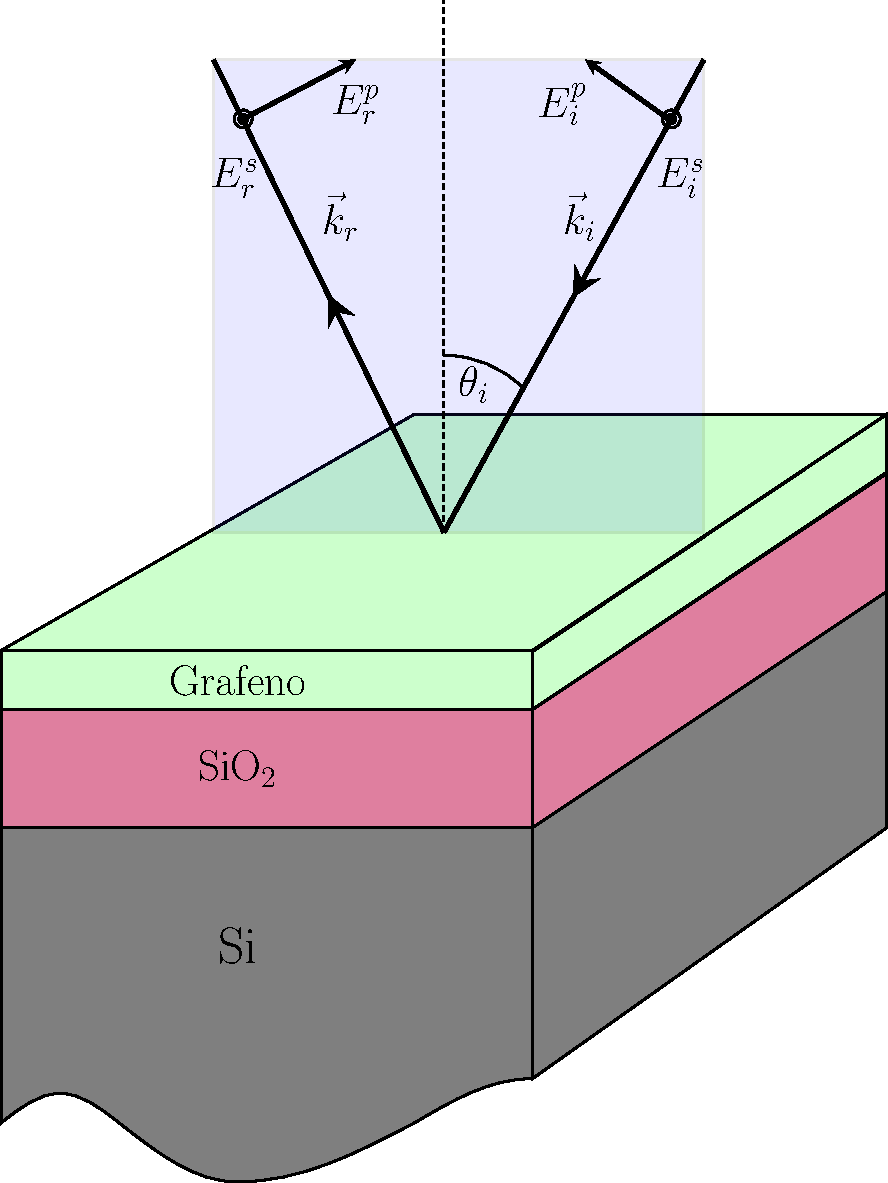
\includegraphics[width=0.45\linewidth]{FIGURES/Experimental_results/Sample.pdf}
	\caption{Carbon allotrope timeline}
	\label{fig:introfig32}
\end{figure}


\section{Graphene nanoribbons}
\begin{figure}
	\centering
	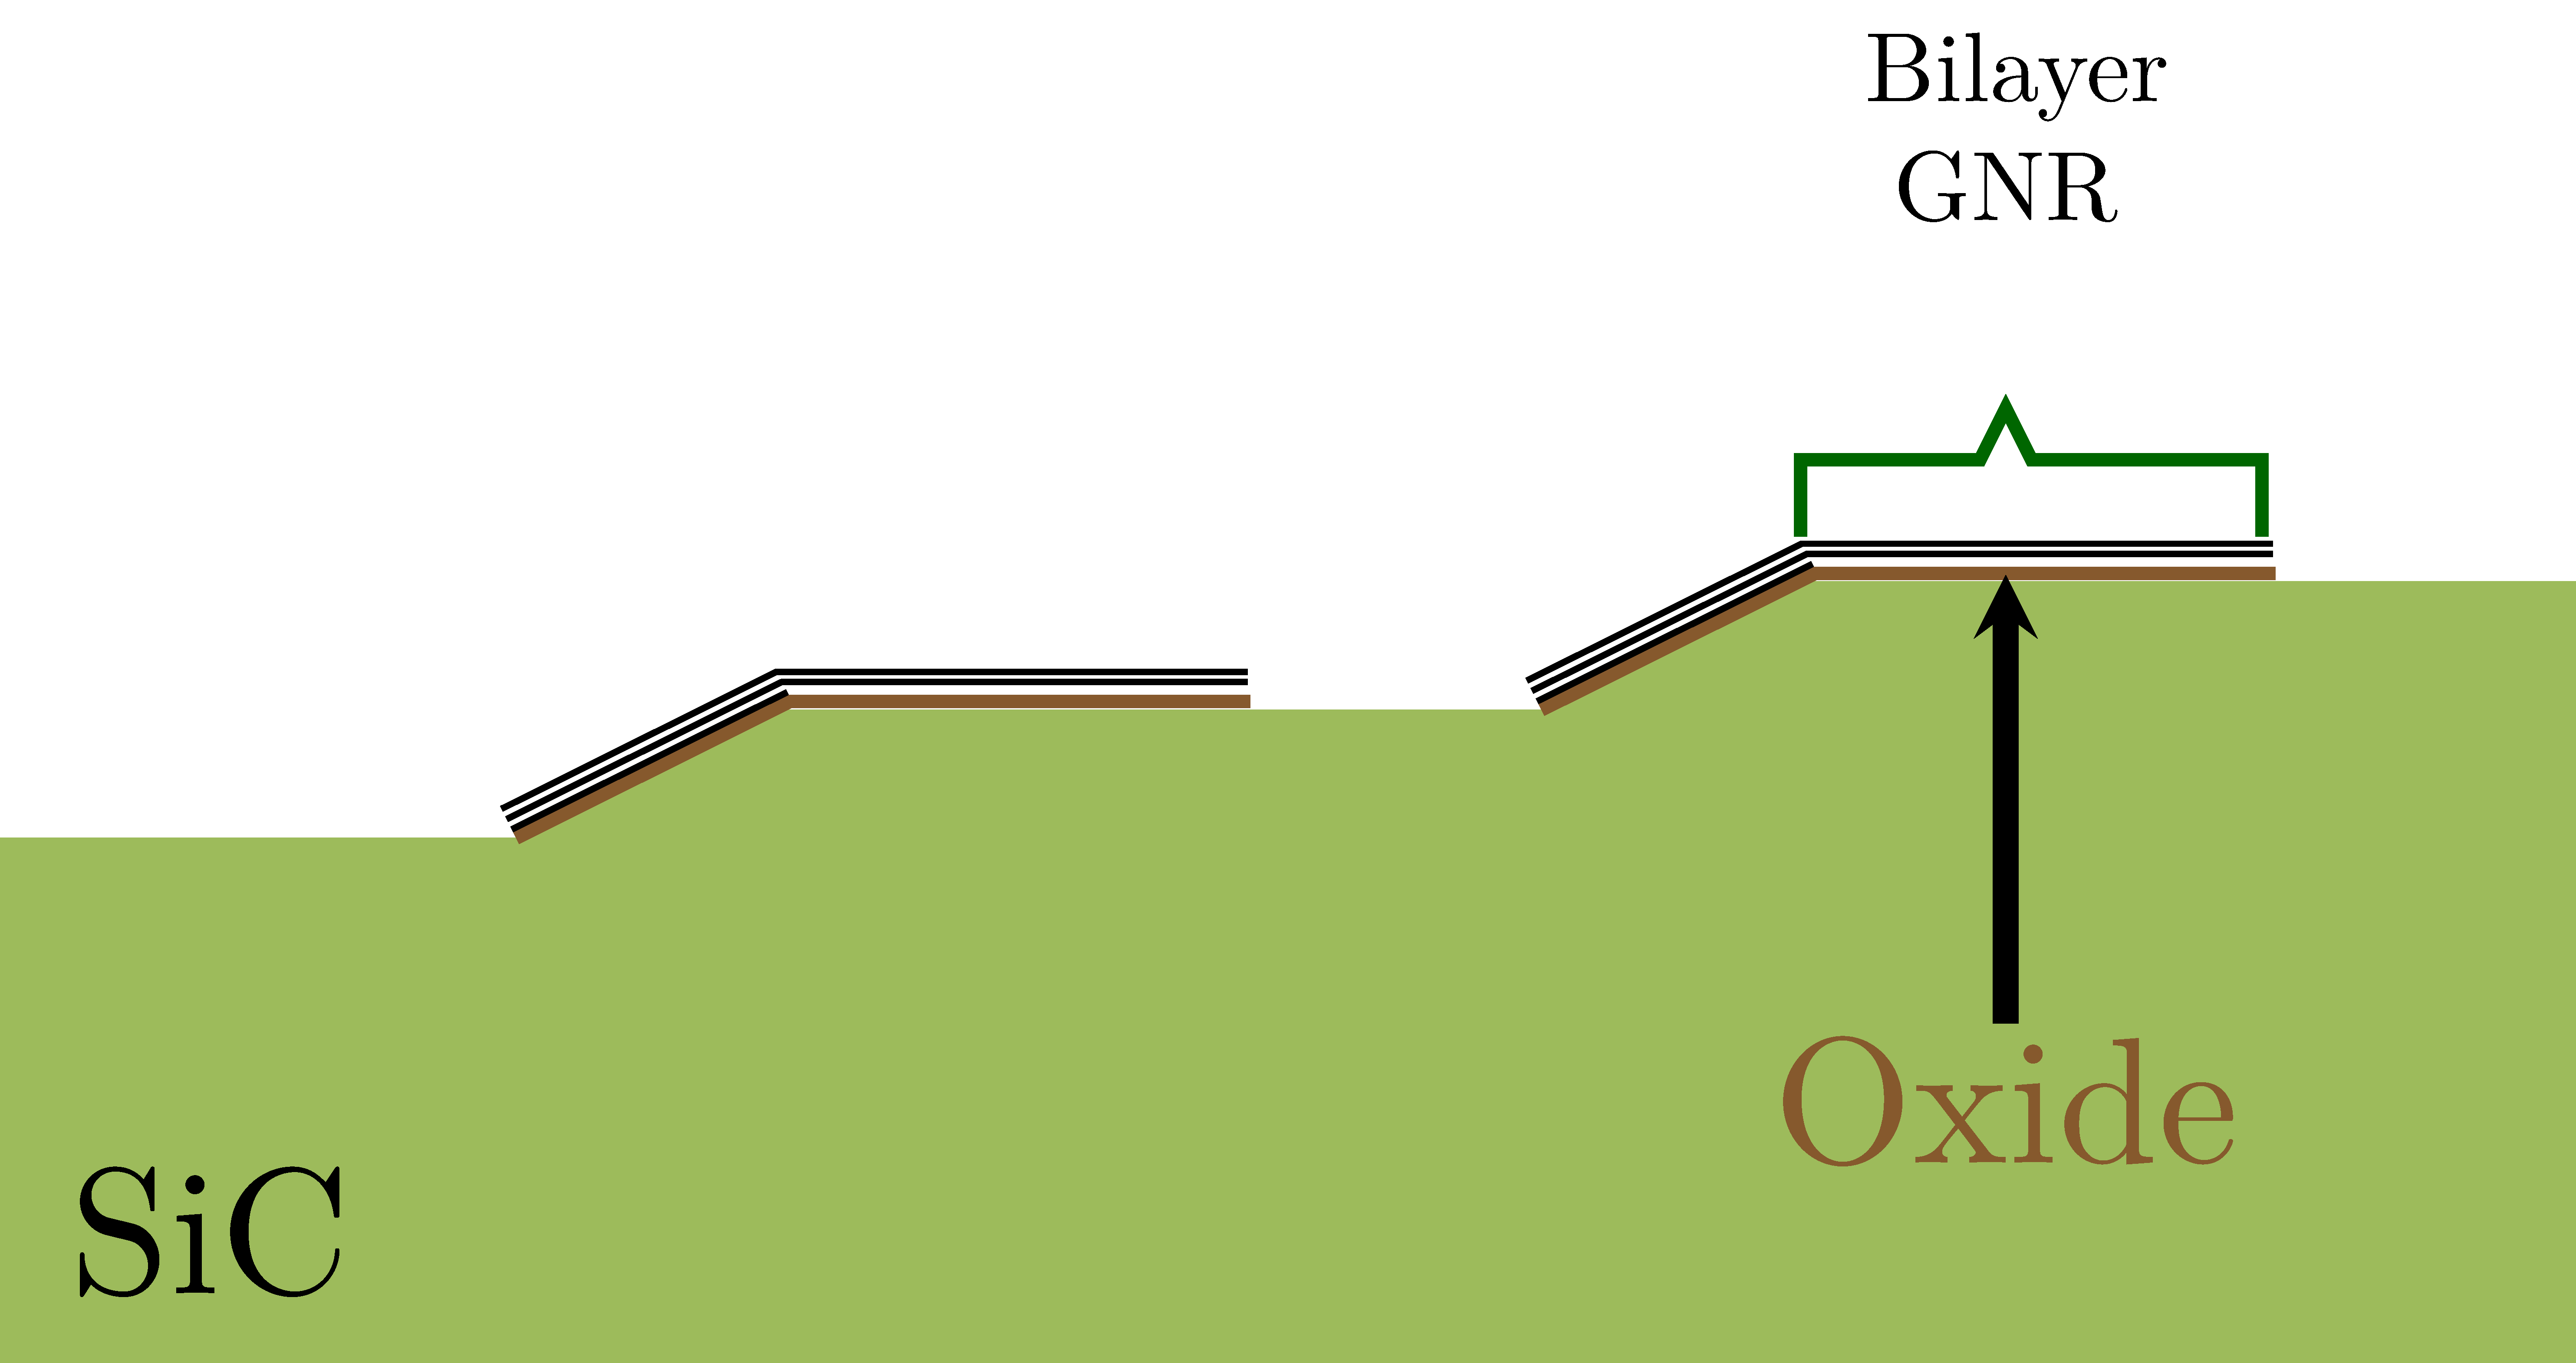
\includegraphics[width=1\linewidth]{FIGURES/Experimental_results/GA.pdf}
	\caption{Carbon allotrope timeline}
	\label{fig:introfig32}
\end{figure}



\begin{figure}
	\centering
	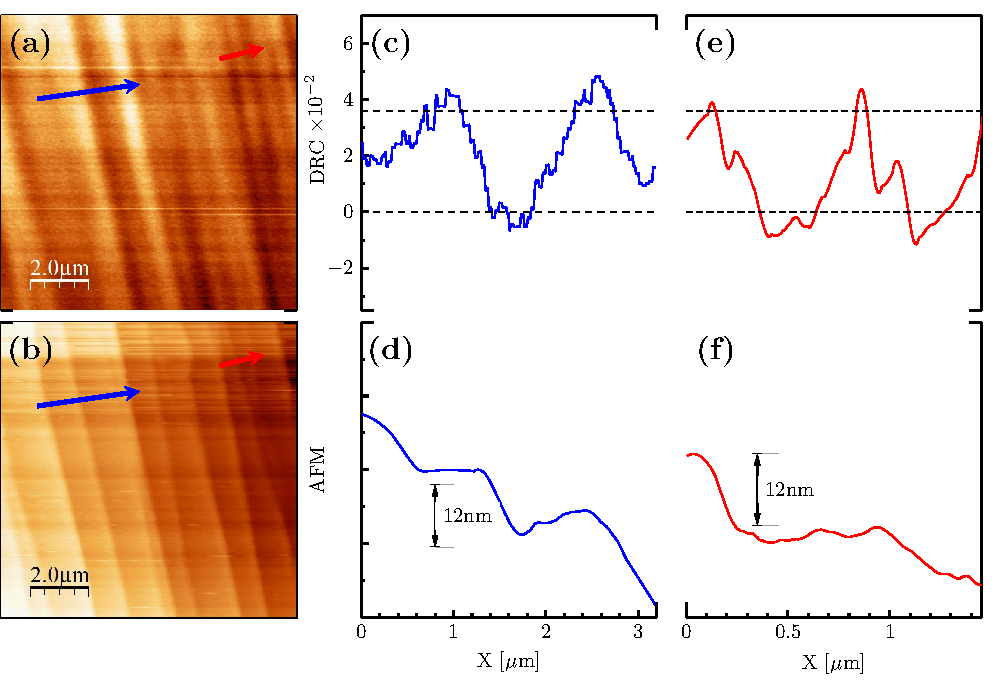
\includegraphics[width=0.75\linewidth]{FIGURES/Experimental_results/FG163R.pdf}
	\caption{Carbon allotrope timeline}
	\label{fig:FG163R}
\end{figure}


\begin{figure}
	\centering
	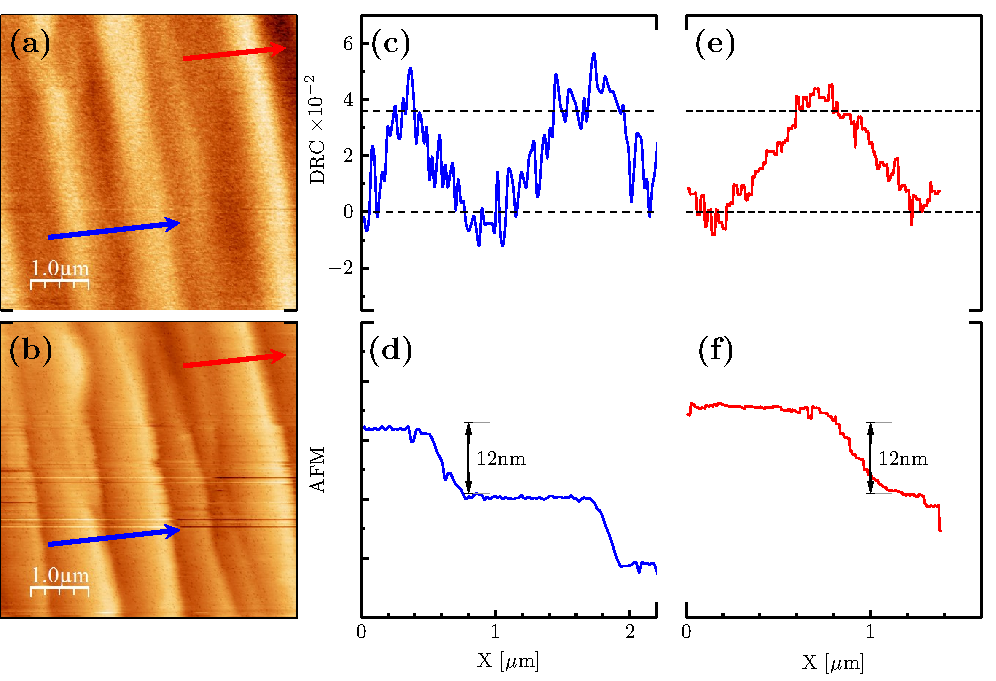
\includegraphics[width=0.75\linewidth]{FIGURES/Experimental_results/FG163R-01.pdf}
	\caption{Carbon allotrope timeline}
	\label{fig:FG163R-01}
\end{figure}


\begin{figure}
	\centering
	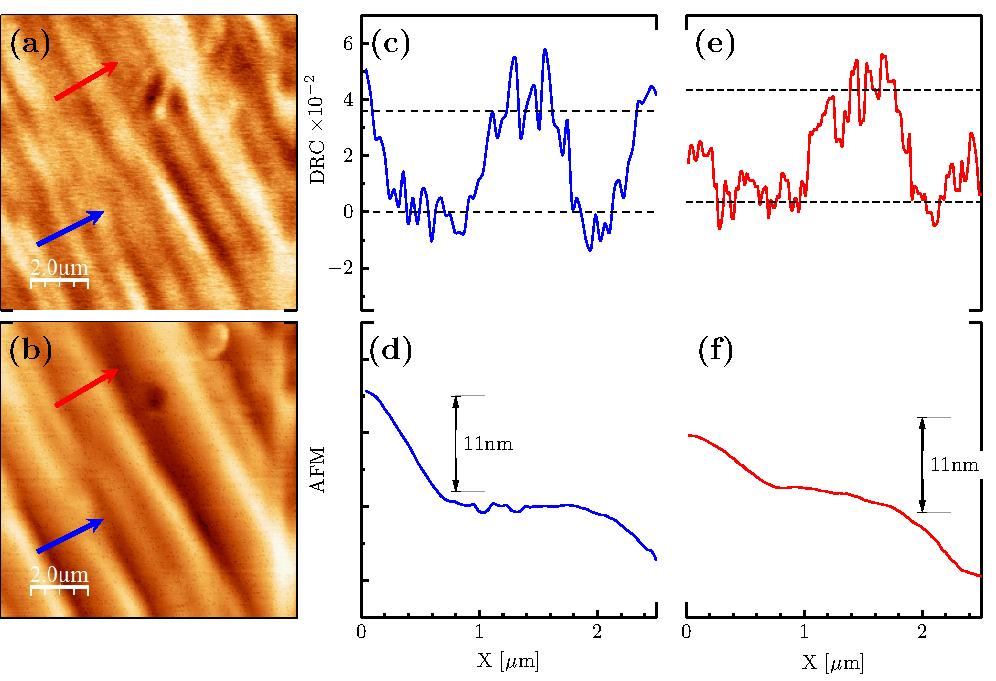
\includegraphics[width=0.75\linewidth]{FIGURES/Experimental_results/FG166L-01.pdf}
	\caption{Carbon allotrope timeline}
	\label{fig:FG166L-01}
\end{figure}


\begin{figure}
	\centering
	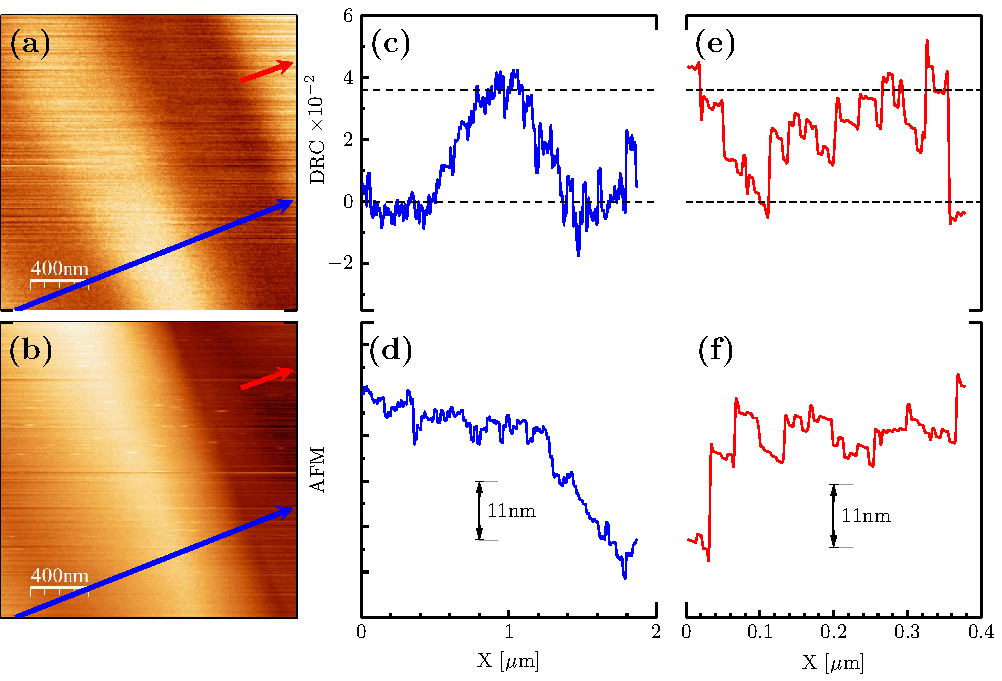
\includegraphics[width=0.75\linewidth]{FIGURES/Experimental_results/FG166L-02.pdf}
	\caption{Carbon allotrope timeline}
	\label{fig:FG166L-02}
\end{figure}


\begin{figure}
	\centering
	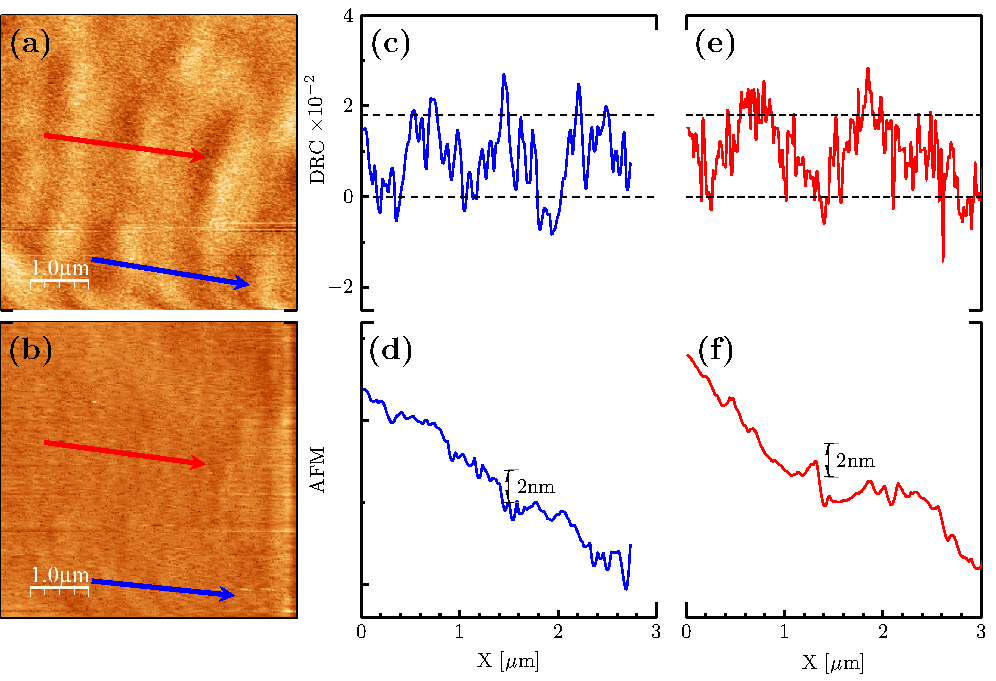
\includegraphics[width=0.75\linewidth]{FIGURES/Experimental_results/FG166R.pdf}
	\caption{Carbon allotrope timeline}
	\label{fig:FG166R}
\end{figure}


\begin{figure}
	\centering
	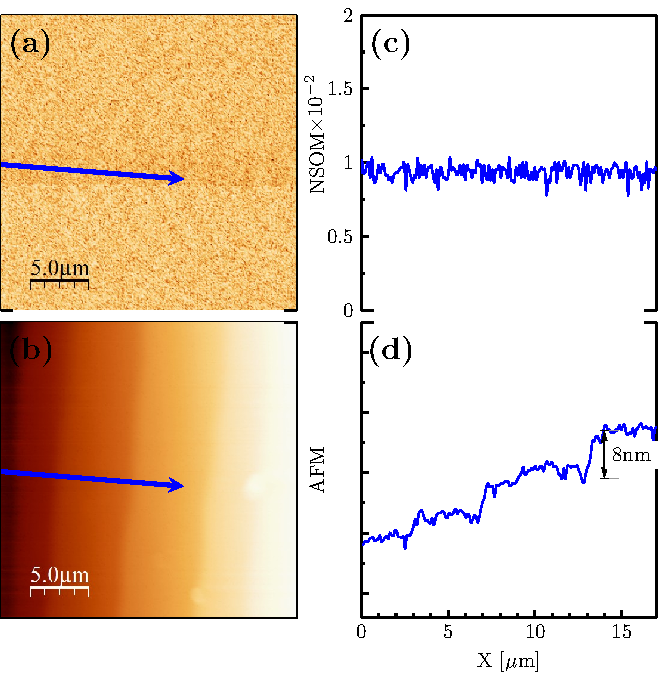
\includegraphics[width=0.75\linewidth]{FIGURES/Experimental_results/FG271.pdf}
	\caption{Carbon allotrope timeline}
	\label{fig:FG271}
\end{figure}

\begin{figure}
	\centering
	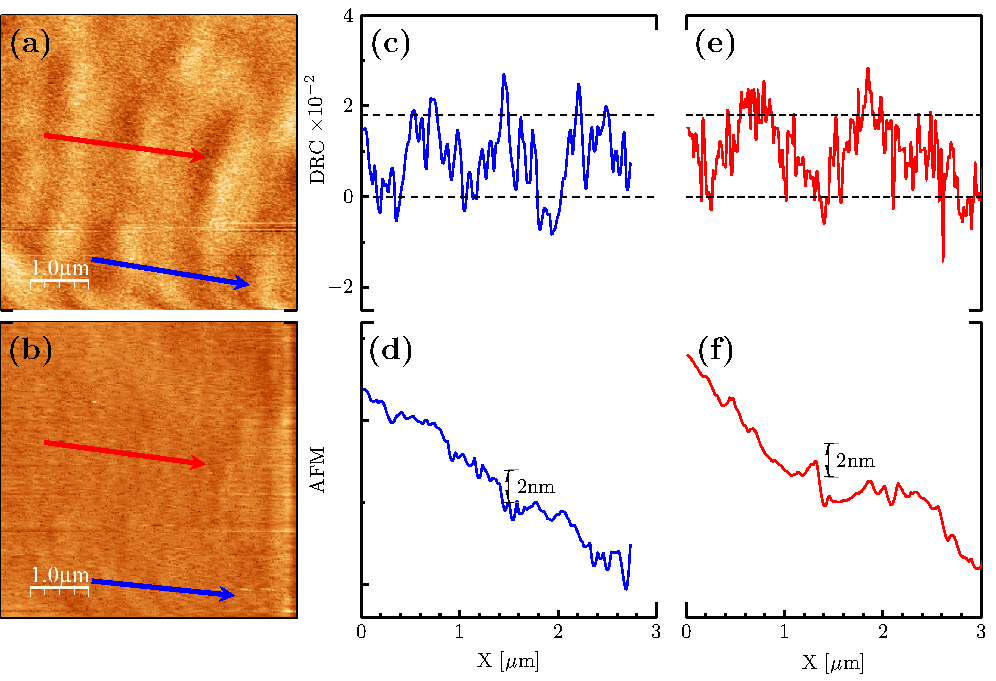
\includegraphics[width=0.75\linewidth]{FIGURES/Experimental_results/FG944-01.pdf}
	\caption{Carbon allotrope timeline}
	\label{fig:FG944-01}
\end{figure}

\begin{figure}
	\centering
	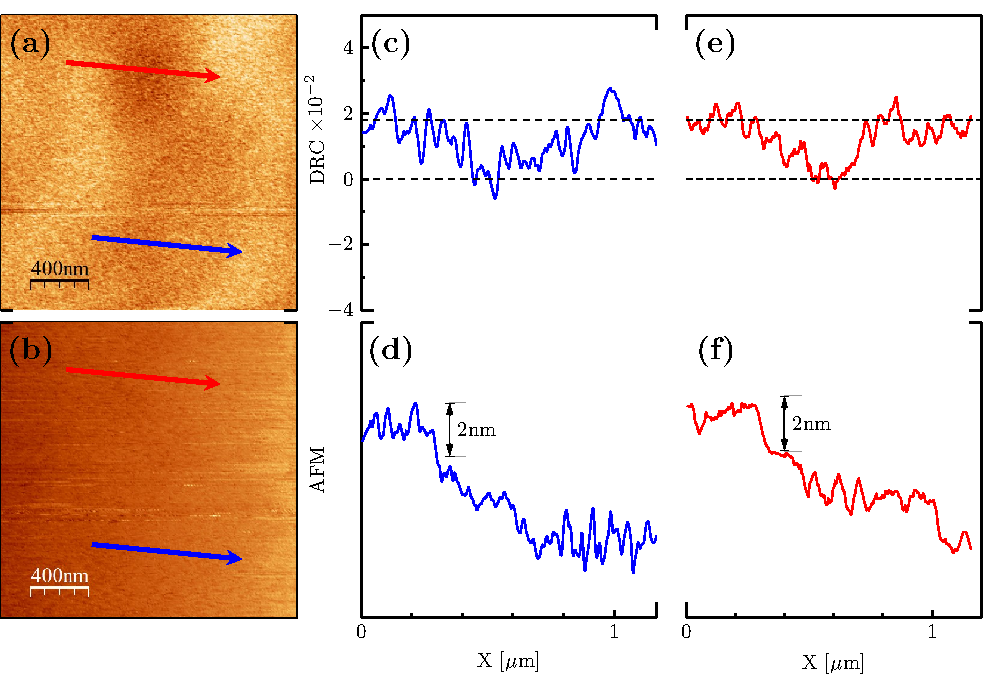
\includegraphics[width=0.75\linewidth]{FIGURES/Experimental_results/FG944-02.pdf}
	\caption{Carbon allotrope timeline}
	\label{fig:FG944-02}
\end{figure}

\begin{figure}
	\centering
	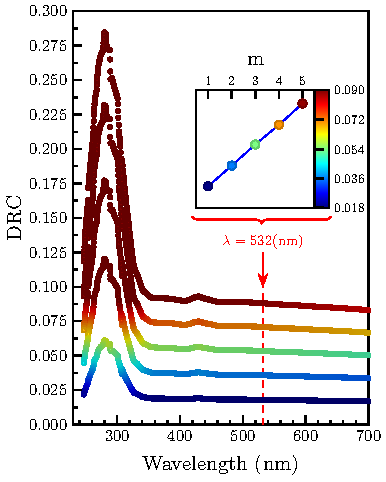
\includegraphics[width=0.75\linewidth]{FIGURES/Experimental_results/image01.pdf}
	\caption{Carbon allotrope timeline}
	\label{fig:DRD}
\end{figure}


\begin{figure}
	\centering
	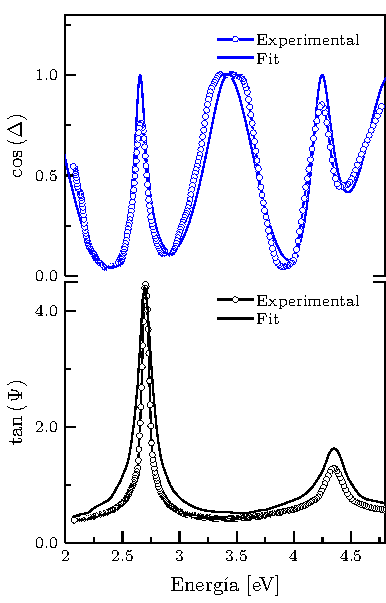
\includegraphics[width=0.75\linewidth]{FIGURES/Experimental_results/Psi_Delta-2.pdf}
	\caption{Carbon allotrope timeline}
	\label{fig:ajusteSiO}
\end{figure}



\subsection{Sample FG163R}

\subsection{Sample FG166L}
\
\subsection{Sample FG166R}


  

